% status: 0
% chapter: TBD

\title{Welcome to Informatica Intelligent Cloud Services}

\author{Sandeep Khandelwal}
\affiliation{%
  \institution{Indiana University}
  \city{Bloomington} 
  \state{IN} 
  \postcode{47408}
  \country{USA}
}
\email{skhande@iu.edu}

% The default list of authors is too long for headers}
\renewcommand{\shortauthors}{S. Khandelwal}

\begin{abstract}
	
In today's world data comes in different format (structured data,
semi-structured data and unstructured data), different volume (data
size is upto hundreds of terabytes) and high velocity (amount of data
getting generated per second is too huge). Also, with the growing
demand of cloud there is massive amount of cloud-based data as well as
on-premise data. This data is sitting ideal in the systems and every
organization has a necessity to integrate such kind of data between
on-premise and cloud-based systems for synchronization, replication or
building warehouse for analysis and reporting purpose. Organization
need to understand the data and get inside about it for business
decision.

Informatica Intelligent Cloud Services (IICS)~\cite{hid-sp18-511-iics}
provide complete suite of integration for such kind of diverse and
unique requirement. Customers can use the features of Informatica
Intelligent Cloud Services (IICS)~\cite{hid-sp18-511-iics} to fulfill
the data related need. This could help to integrate data in different
format like text file, csv files, databases, on-premise ERP systems,
cloud-based systems and many more.

\end{abstract}

\keywords{hid-sp18-511, IICS, Informatica, ETL, Data Integration}


\maketitle


\section{Introduction}

Informatica Intelligent Cloud Services (IICS)~\cite{hid-sp18-511-iics}
is built on micro service architecture and provide capability of data
integration between cloud-based and on-premise systems. Informatica
Intelligent Clod Services IICS~\cite{hid-sp18-511-iics} provide
integration capability in four areas mainly Integration Cloud, Data
Quality and Governance Cloud, Master Data Management Cloud, and Data
Security Cloud.

Informatica Intelligent Cloud Services (IICS)~\cite{hid-sp18-511-iics}
processing engine which is called integration engine could be run in
the cloud or on-premise. In case of on-premise processing customer has
to download the integration agent and use that for the processing
logic.

Informatica Intelligent Cloud Services (IICS)~\cite{hid-sp18-511-iics}
comes under the category of Integration platform as aa service
(iPAAS)~\cite{hid-sp18-511-ipaas}

As Informatica Intelligent Cloud Services
(IICS)~\cite{hid-sp18-511-iics} is in the cloud hence customer need
not to worry about the maintenance or upgrade of the software. The
underlying hardware maintenance, OS patching, software upgrade
etc. maintenance tasks will be performed by Informatica and customer
has to focus only on the business logic. There are different type of
pricing options available for the
product!\cite{hid-sp18-511-iics-pricing}. Customer has the option to
use pricing model as per the requirement and need.

As Informatica Intelligent Cloud Services
(IICS)~\cite{hid-sp18-511-iics} provide 30-day free trial. This free
trial could be used to evaluate the product and make the decision
based on the features provided by the product.

Informatica provide very robust easily accessible Global Customer
Support (GCS)~\cite{hid-sp18-511-gcs}service. This team is a set of
dedicated people who are ready to help in resolving the questions
related to pricing, technical queries or any other kind of help.

\section{Integration Cloud}

Integration Cloud~\cite{hid-sp18-511-iics} product provide easy to use
framework and designer for developing data integration engine between
on-premise and cloud-based systems. It provide easy to develop
interface for fast and easy development of integration logic. It has
high performance data transformations including filter, router,
expression etc. to massage the data in desired format. These
transformations are ready to use and can be used in any data
processing. Each transformation has different customization option
which customer could use as per the requirement. It has push-down
optimization feature for fast performance to move the data processing
logic to database itself instead of retrieving the data and performing
the operations in Integration
Cloud~\cite{hid-sp18-511-iics}. push-down optimization feature is
really helpful to improve the performance of the integration logic. It
provide the connectivity between cloud based databases like Amazon
Redshift~\cite{hid-sp18-511-aws-redshift}, Microsoft Azure SQL Data
Warehouse~\cite{hid-sp18-511-ms-azure-sql}, Google
BigQuery~\cite{hid-sp18-511-google-bigquery}, and
Snowflake~\cite{hid-sp18-511-snowflake} and on-premise legacy
databases for the integration between these systems.

\subsection{Easy to use interface}

Integration Cloud~\cite{hid-sp18-511-iics} provide easy to use, common
framework for developers and administrators. This interface is
consistent across all products. As the development framework is in the
cloud hence it could be accessed from anywhere and anytime.

\subsection{Fast development}

Integration Cloud~\cite{hid-sp18-511-iics} provide pre-built logic
which customer can use and customize as per their need. There is no
need to develop the logic from scratch. This helps in fast
development. Time to market is a concern in today's IT industry and
availability to deliver in the market fast is very important. The
pre-built logic helps organization to deliver in the market very
fast. Customer can prepare the logic from scratch too if they want.

\subsection{Changed Data Capture}

Integration Cloud~\cite{hid-sp18-511-iics} has changed data capture
functionality to capture only the changed data at source system and
replicate to downstream systems. This way replication is fast and as
only changed data gets processed instead of bulky process of moving
the entire data from source to downstream systems.

\subsection{Access Policy}

Integration Cloud~\cite{hid-sp18-511-iics} has access policy to
determine who can access and what. Administrators can easily provide
the permission to different project and folders based on the
requirement to different users using easy graphical user
interface. There could be multiple projects and different set of
people could be working on those projects. There is a need to separate
the access across team so one team can not access the work done by
others. Also, there is a need to separate the access between lower
environments and higher environments. Developers can run the
integration logic in development environment but they should not be
able to run the integration engine in higher environments. Access
policy is very important in any organization and Integration
Cloud~\cite{hid-sp18-511-iics} provide easy way to do this.

\subsection{Amazon S3 integration}

Integration Cloud~\cite{hid-sp18-511-iics} provide tool to move the
data from flat files on-premise systems to cloud based Amazon file
store (S3)~\cite{hid-sp18-511-aws-s3}. This is useful for the mass
ingestion of the data. Multiple set of files could be move to S3 in a
single click.

\subsection{Development framework}

Integration Cloud~\cite{hid-sp18-511-iics} provide easy to use
designer to develop the integration logic and monitor tool to check
the progress of integration flow.

\subsection{Application integration at run time}

Integration Cloud~\cite{hid-sp18-511-iics} provide functionality to
integrate cloud based application like
Salesforce~\cite{hid-sp18-511-salesforce} with on-premise systems like
databases in real time. Real time integration happens through RESTful
APIs. Developers have to provide the RESTful APIs to be called when an
event occurs in Salesforce~\cite{hid-sp18-511-salesforce} system like
customer added, order made etc. RESTFul APIs will be called once such
event occur which have the logic to push the data to legacy systems
like databases. All this happen in the real time. There are few
security related configuration that organization have to provide.

\subsection{Business to Business integration}

Integration Cloud~\cite{hid-sp18-511-iics} provide transformation to
deal with industry standards format like Electronic Data Exchange
(EDI)~\cite{hid-sp18-511-edi}. Customer can easily leverage the
industry standards with legacy systems to understand or transform the
data. B2B tools provide tool for easy integration of industry standard
formats.

\section{Data Quality and Governance Cloud}

With the massive amount of data available in today's world it is very
important that we have access to the clean and quality
data. Information can be retrieved and analysis could be performed
only if we have the good quality data with we could rely upon and
trust. Incorrect data means incorrect analysis and ultimately
incorrect decision which might lead to business loss. Data Quality and
Governance Cloud~\cite{hid-sp18-511-iics} product provide tools to
visualize the data quality issues present in the data and fix them in
automated way. It also provide tools to verify and correct the common
data related issues like update the address of people and organization
based on the available address database, update the email addresses
based on the common email address rules, update the phone numbers
based on the phone rules etc. Data Quality is very first and important
process in data analyis.

\section{Master Data Management Cloud}

Master Data Management Cloud~\cite{hid-sp18-511-iics} provide 360 view
of customer data by consolidating the customers data from different
systems. This is very important for any organization to get the full
view of the customer in a holistic way and make the decisions
accordingly. Customer data is normally stored in different systems
having different perspective. The data could be on
Salesforce\cite{hid-sp18-511-salesforce} and it could be on legacy
on-premise systems like database. This kind of data which is stored at
multiple places doesn't server any purpose unless it is integrated and
analyzed.

\section{Data Security Cloud}

Testing is a real need for validating the application before it could
be used for the real purpose. No one is ready to use any system until
it's authenticity and functionality is proven. However, providing live
data for testing is a risk and data could be compromised. Data breach
might lead to lot of compliance issues and might risk the position of
the organization and ultimately business loss. Hence, there is a real
need to provide the real live look like real data without compromising
it. Data Security Cloud\cite{hid-sp18-511-iics} provide tool to mask
the data before sharing it with anyone which will convert the data
without loosing the shape of the data

In Figure~\ref{f:iics-products}\cite{hid-sp18-511-iics} see the
architecture of Informatica Integration Cloud Services
(IICS)~\cite{hid-sp18-511-iics}.

\section{API Management}

Customer could develop RESTFul APIs using Informatica Intelligent Cloud Services (IICS)~\cite{hid-sp18-511-iics} framework. Informatica Intelligent Cloud Services (IICS)~\cite{hid-sp18-511-iics} framework allows easy debugging, API lifecycle management, API access security, API usage dashboard~\cite{hid-sp18-511-iics-pricing}. Customer could develop APIs for the data integration, replication and similar data integration features which end user could consume in various applications. The metadata about the APIs is stored in a well structured format that developer could easily locate and use them. It complete complete suite for the API development for the end consumers.

\section{Cloud Integration Hub}
Informatica Intelligent Cloud Services (IICS)~\cite{hid-sp18-511-iics} provide Cloud Integration Hub~\cite{hid-sp18-511-iics-hub} which could be integrate to on-premise and cloud systems. The services are self serviced, efficient and cost effective. It provide nice integration of Salesforce~\cite{hid-sp18-511-salesforce} system with on-premise systems

\begin{figure}[!ht]
	\centering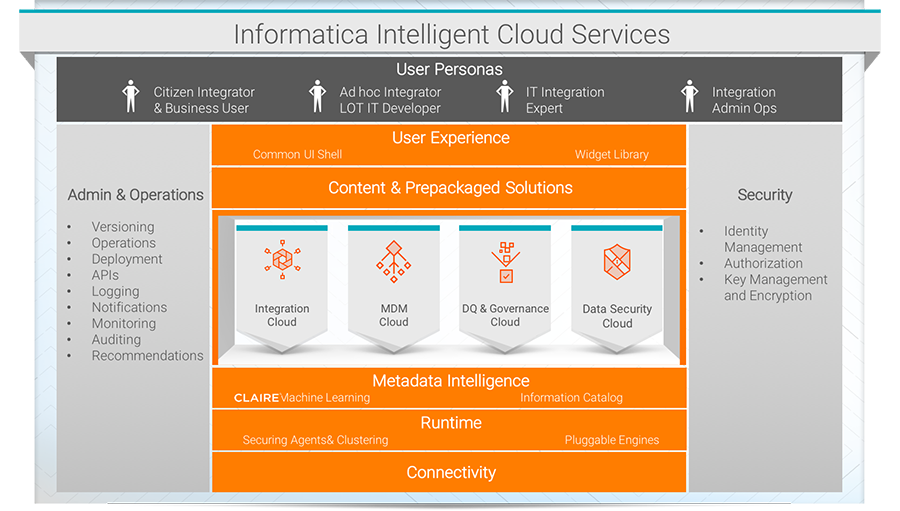
\includegraphics[width=\columnwidth]{images/iics-diagram.png}
	\caption{IICS architecture}\label{f:iics-products}
\end{figure}

\begin{acks}

The author would like to thank Dr.~Gregor~von~Laszewski for his
support and suggestions to write this paper.

\end{acks}

\bibliographystyle{ACM-Reference-Format}
\bibliography{report} 
